\section{Overview}

Given the raw TV broadcasts, each shot must be automatically tagged with the name(s) of people who can be both seen as well as heard in the shot along with the confident score. The list of people is not known apriori and their names must be discovered from video text overlay or speech transcripts~\cite{bredin2016mediaeval}. 
%
To this end, a video must be segmented in an unsupervised way into homogeneous segments according to person identity, like  speaker diarization and face diarization, to be combined with the extracted names.
% . Combined with the extracted names,  audio-visual person diarization makes it possible to identify people in videos. % \cite{Gay:Frontiers:2016}.
%

%\begin{figure}[tb]
%\centering
%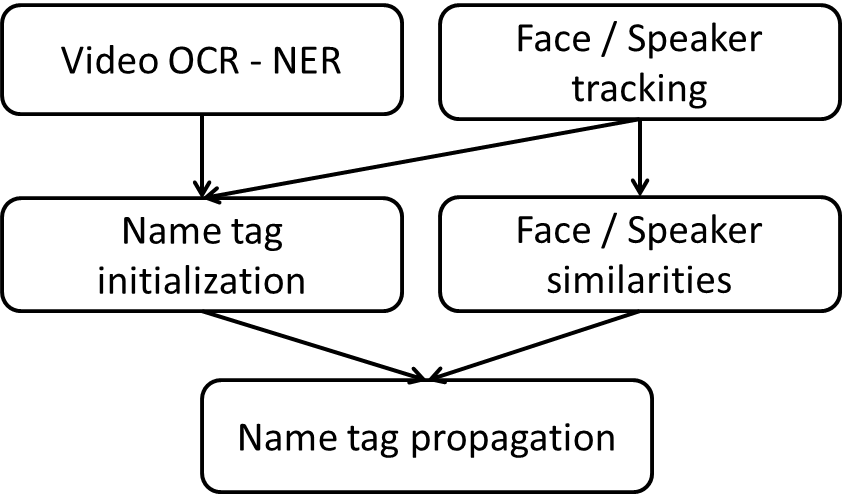
\epsfig{file=diagram.png,width=70mm}
%\vspace*{-3mm}
%\caption{Architecture of our system}
%\vspace*{-3mm}
%\label{fig:pipeline}
%\end{figure}

The overall system is illustrated in Fig.~\ref{fig:pipeline}. It consists of  4 main parts: video optical character recognition (OCR) and named entity recognition (NER), face diariation, speaker diarization, and fusion naming. Each of these parts will be described in the following sections.

\endinput
